\subsubsection{MLP Fact-Storage Capacity}
\label{app:exp:section4:capacity}
We estimate the MLP fact-storage capacity in Figure~\ref{fig:sketched_k2_sweeps}c by binary-searching over hidden width $m$ at fixed embedding dimension $d$ and fact count $F$.
We sweep over
\[
d\in\{64,90,128\},
\qquad
\alpha:=F/d^2\in\{1/32,1/16,1/8,1/4,1/2,3/4,1\}.
\]
For each $(\text{method},d,\alpha)$ tuple, we generate a random-permutation fact set and sample key and value embeddings from the unit sphere.
We then binary-search for the smallest hidden width $m$ that attains 100\% fact storage on the sampled fact set and report the corresponding parameter count $W$.
We compare GD-trained bilinear MLPs, our sketched-$K_2$ Hebbian construction (with and without whitening, and our data-dependent kernel variant), and the NTK baseline from~\citet{nichani2024understandingfactualrecalltransformers}, as described in Appendix~\ref{app:exp:mlp-variants}.

\subsubsection{Margin Sweeps}
\label{app:exp:section4:margins}
We use the same bilinear sketched-$K_2$ construction for the isotropic margin sweeps in Figure~\ref{fig:sketched_k2_sweeps}b, as well as for the arbitrary-geometry comparisons summarized in Table~\ref{tab:2x2}.

\paragraph{Isotropic keys and values.}
\label{app:exp:section4:iso-iso}
For the isotropic keys and isotropic values sweeps supporting Appendix~\ref{app:theory:margin_bounds:rkrv}, we sample unit-norm spherical keys and values from a random-permutation fact set, vary either $F$ or $m$, and construct the MLP at each point.
We then compare the measured minimum margin with the theoretical prediction (\Cref{eq:app:rkrv:sketchedk2_full}).
The $F$-sweep (exact $K_2$) uses $d=32$, $m=512$, $F\in[32,2048]$ (30 log-spaced points, 5 seeds).
The $F$-sweep (bilinear sketched-$K_2$) uses $d=64$, $m=512$, $F\in[32,512]$ (30 log-spaced points, 5 seeds).
The $m$-sweep (bilinear bilinear sketched-$K_2$) uses $d=64$, $F=256$, $m\in[64,1024]$ (30 log-spaced points, 5 seeds).

\begin{figure}[h]
\centering
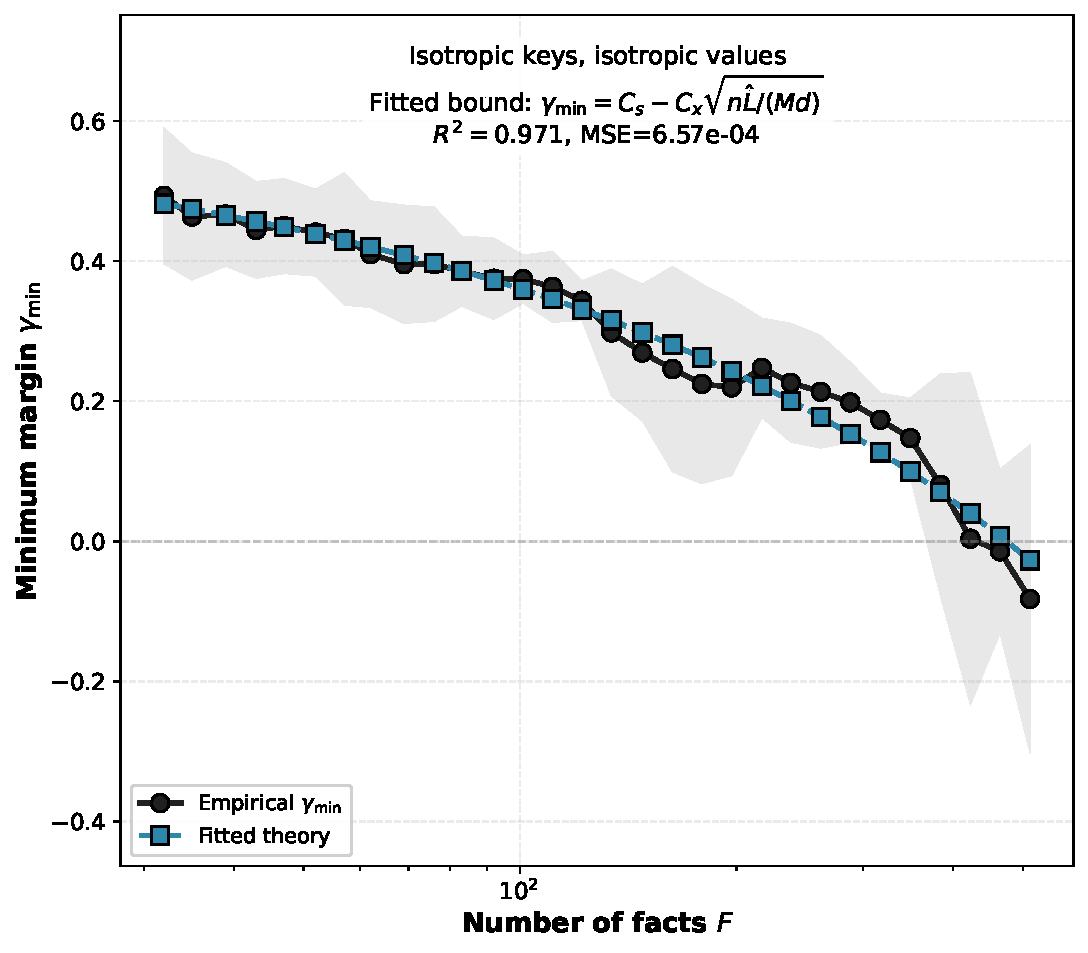
\includegraphics[width=0.60\linewidth]{appendix/theory/rf_F_d64_30pts_rkrv_F.pdf}
\caption{\textbf{Margin scaling with number of facts (isotropic setting).}
Minimum margin of bilinear sketched-$K_2$ MLPs decreases with the number of stored facts $F$, following the predicted scaling from \Cref{eq:app:rkrv:sketchedk2_full}. The empirical margin closely tracks the theoretical bound across the $F$-sweep with $d=64$, $m=512$.}
\label{fig:app:rf-f-sweep}
\end{figure}

\paragraph{Arbitrary keys, isotropic values.}
\label{app:exp:section4:anisotropic-keys}
For the arbitrary-key sweep supporting Appendix~\ref{app:theory:margin_bounds:akrv}, we start from spherical keys and apply a rank-1 spike transform
\[
\mathbf{k}_{i}'
=
\frac{\mathbf{k}_{i} + \beta \langle \mathbf{k}_{i}, \mathbf{u}\rangle \mathbf{u}}
{\|\mathbf{k}_{i} + \beta \langle \mathbf{k}_{i}, \mathbf{u}\rangle \mathbf{u}\|_2},
\]
where $\mathbf{u}\in\mathbb{S}^{d-1}$ is fixed within a sweep and $\beta\ge 0$ controls the anisotropy strength.
As $\beta$ increases, the keys crowd along $\mathbf{u}$, increasing the key-side quantities entering the bound, especially $E_{K}$.
Values remain isotropic, sampled uniformly from the unit sphere.
At each $\beta$, we construct the MLP, measure $\gamma_{\min}$, and compare it against the theorem, plug-in, and heuristic predictions for the resulting key geometry (\Cref{eq:app:akrv:thm}).
We use $d=64$, $F=128$, $m=512$, $\beta\in[0,5]$.

\paragraph{Isotropic keys, arbitrary values.}
\label{app:exp:section4:anisotropic-values}
For the arbitrary-value sweep supporting Appendix~\ref{app:theory:margin_bounds:rkav}, we keep the keys isotropic and apply the same rank-1 spike transform to the values:
\[
\mathbf{v}_{i}'
=
\frac{\mathbf{v}_{i} + \beta \langle \mathbf{v}_{i}, \mathbf{u}\rangle \mathbf{u}}
{\|\mathbf{v}_{i} + \beta \langle \mathbf{v}_{i}, \mathbf{u}\rangle \mathbf{u}\|_2}.
\]
Again $\mathbf{u}$ is fixed within a sweep and $\beta$ is the control parameter. This changes the value-side quantities $V_{\min}$, $B_{Y}$, and $E_{v}$ while preserving unit norm.
Keys remain isotropic, sampled uniformly from the unit sphere.
At each $\beta$, we rebuild the MLP, measure the empirical decoding margin, and compare it against the corresponding theorem, plug-in, and heuristic predictions (\Cref{eq:app:rkav:thm}).
We use $d=64$, $F=128$, $m=512$, $\beta\in[0,10]$.

\paragraph{Arbitrary keys and values.}
\label{app:exp:section4:anisotropic-keys-values}
For the fully structured sweep supporting Appendix~\ref{app:theory:margin_bounds:akav}, we apply the same rank-1 spike model to both keys and values, using the same spike strength $\beta$ and fixed direction $\mathbf{u}$:
\[
\mathbf{e}_{i}'
=
\frac{\mathbf{e}_{i} + \beta \langle \mathbf{e}_{i}, \mathbf{u}\rangle \mathbf{u}}
{\|\mathbf{e}_{i} + \beta \langle \mathbf{e}_{i}, \mathbf{u}\rangle \mathbf{u}\|_2},
\qquad
\mathbf{e}_{i}\in\{\mathbf{k}_{i},\mathbf{v}_{i}\}.
\]
This setting makes key crowding and value interference vary coherently, which is the regime where the coupling factor $\kappa$ emerges.
For each $\beta$, we recompute the geometric summary statistics entering the deterministic bound and compare the measured margin against the theorem, plug-in, and heuristic predictions, focusing on the composite cross-talk scale $\sqrt{E_K}\sqrt{E_v}\,\kappa$ (\Cref{eq:app:akav:thm}).
We use $d=64$, $F=128$, $m=512$, $\beta\in[0,3.35]$.

\begin{figure*}[t]
\centering
\begin{subfigure}[t]{0.32\linewidth}
\centering
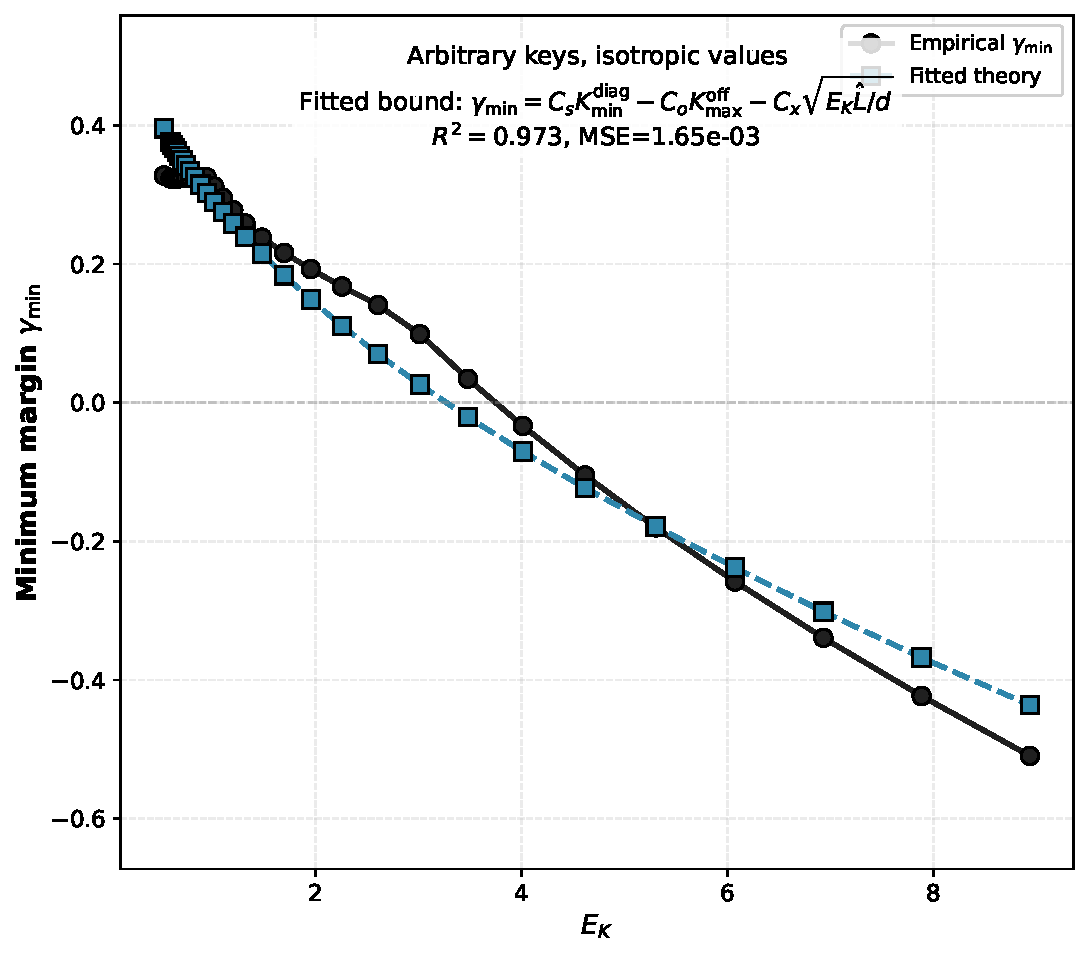
\includegraphics[width=\linewidth]{sections/section_4_hebbian_kernel_mlps/figs/beta_keys_F128_bmax35_akrv_beta.pdf}
\caption{Arbitrary keys, isotropic values ($\beta$-sweep). As $\beta$ increases, key crowding grows and the measured margin tracks the theoretical bound via key-geometry terms $K_{\min}^{\mathrm{diag}}$, $K_{\max}^{\mathrm{off}}$, and $E_K$.}
\label{fig:app:beta-sweep-akrv}
\end{subfigure}\hfill
\begin{subfigure}[t]{0.32\linewidth}
\centering
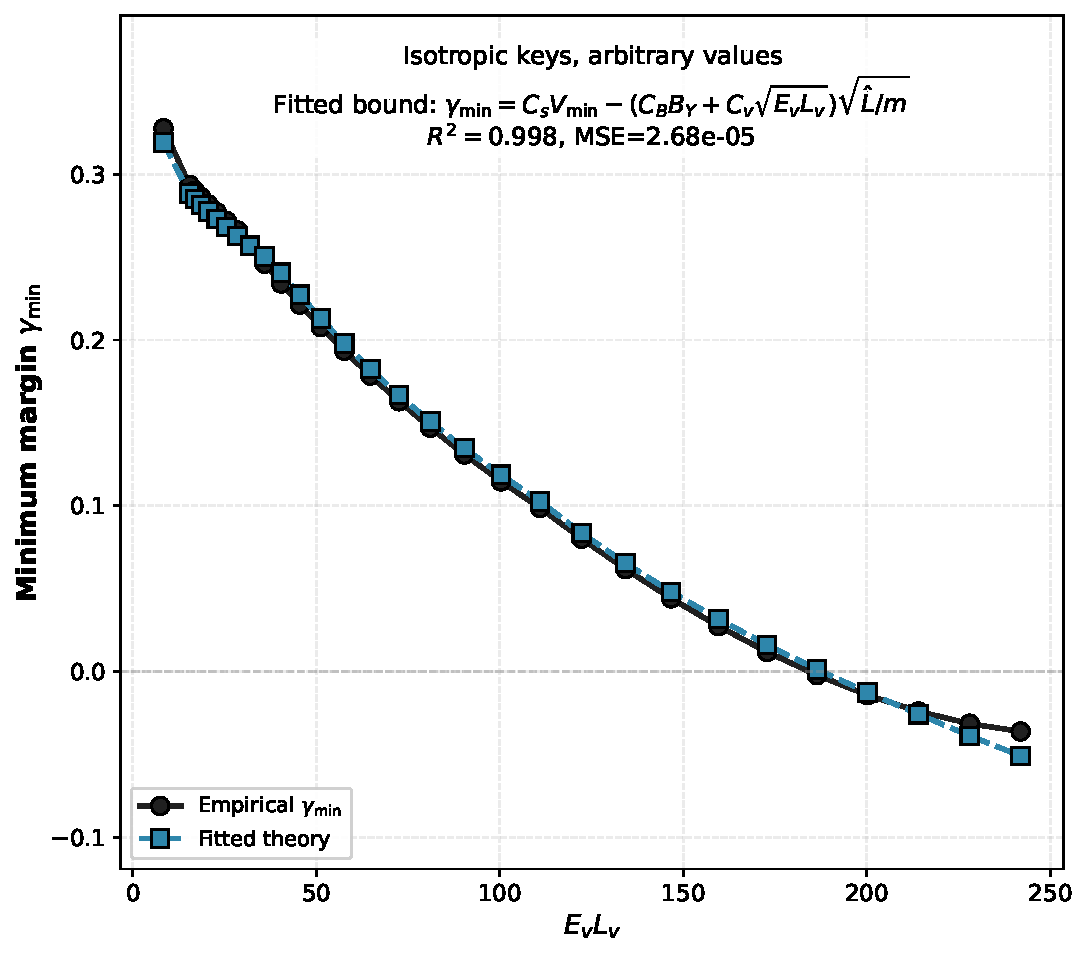
\includegraphics[width=\linewidth]{sections/section_4_hebbian_kernel_mlps/figs/beta_values_F128_bmax10_rkav_beta.pdf}
\caption{Isotropic keys, arbitrary values ($\beta$-sweep). Increasing $\beta$ concentrates values and the margin closely follows the bound through value-geometry terms $V_{\min}$, $B_Y$, and $E_v$.}
\label{fig:app:beta-sweep-rkav}
\end{subfigure}\hfill
\begin{subfigure}[t]{0.32\linewidth}
\centering
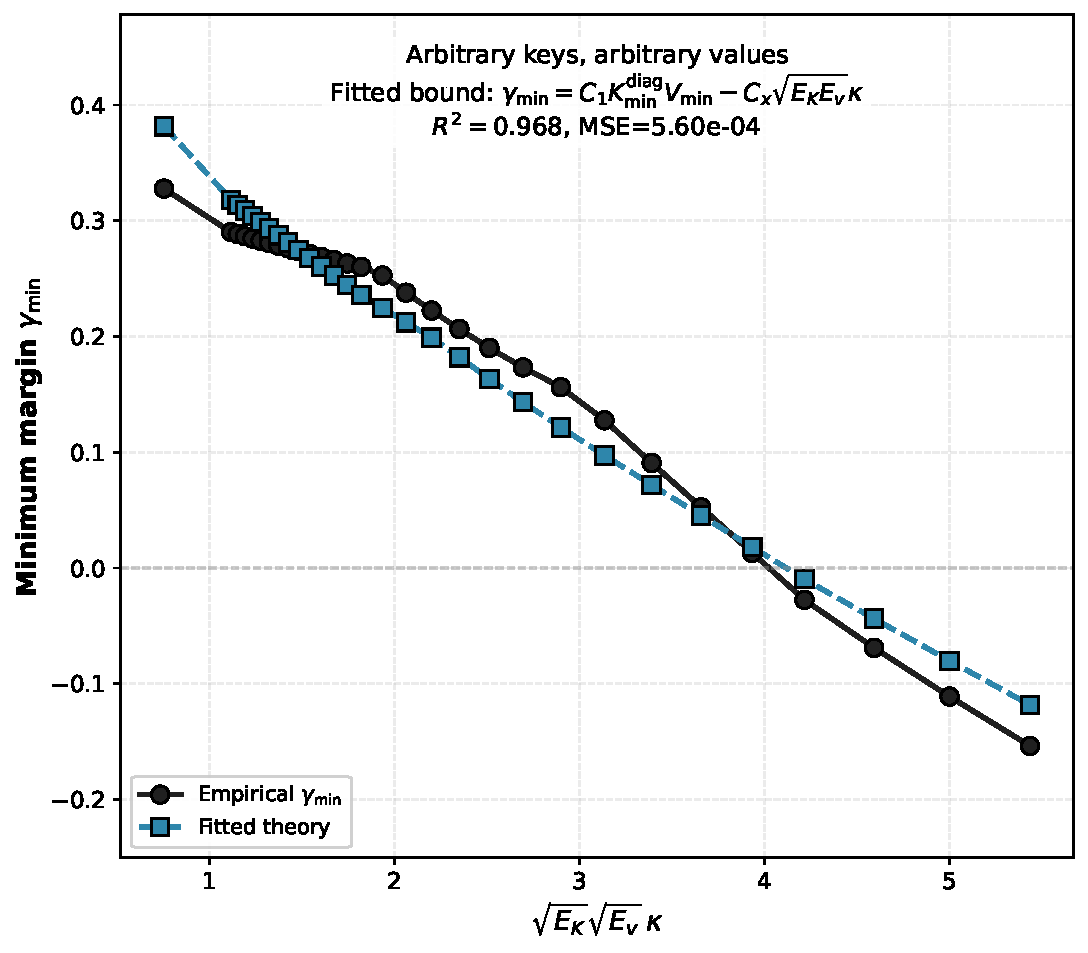
\includegraphics[width=\linewidth]{sections/section_4_hebbian_kernel_mlps/figs/beta_both_F128_bmax335_akav_beta.pdf}
\caption{Arbitrary keys and values ($\beta$-sweep). Both geometries are spiked simultaneously; the margin degradation is governed by the composite cross-talk scale $\sqrt{E_K}\sqrt{E_v}\,\kappa$, matching the deterministic bound.}
\label{fig:app:beta-sweep-akav}
\end{subfigure}
\caption{\textbf{Margin $\beta$-sweeps across arbitrary key/value geometry regimes.}
Each panel applies a rank-1 spike transform with strength $\beta$ to the keys (left), values (middle), or both (right), using $F=128$ facts.
In all three cases the theoretical bound tracks the empirically measured minimum margin ($R^2\geq0.95$), validating the margin decomposition of \Cref{eqn:margin-decomposition} and the geometric summary statistics of \Cref{tab:2x2}.
The arbitrary keys and values plot uses the raw summary-statistic form of \Cref{thm:combined-deterministic}, which is equivalent to the penalty-statistic general margin/capacity bound in \Cref{cor:optimal-fact-storage-capacity-arb-formal} of the main text.}
\label{fig:app:beta-sweeps}
\end{figure*}
